\chapter*{\large Ejemplos}
\addcontentsline{toc}{chapter}{\large Ejemplos}

\pagestyle{fancy}
\lhead{}
\chead{}
\rhead{Ejemplos}
\lfoot{}
\cfoot{}
\rfoot{\thepage}
\renewcommand{\headrulewidth}{0.4pt}
%\renewcommand{\footrulewidth}{0.4pt}
 \vspace{-1cm}


% \todo[inline,color={red!100!green!33},bordercolor=red,linecolor=red]{A todonote placed in the text}

\section*{\large Comentarios}
\addcontentsline{toc}{section}{\large Comentarios}

\comentario{ \bf Ejemplo de como hacer un comentario de textos, para el código se usa el paquete verbatim}

\section*{\large Uso del comando verbatim}
\addcontentsline{toc}{section}{\large Uso del comando verbatim}

\begin{verbatim}
    $node = xmlrpc('http://empleos.mentor/services/xmlrpc', 'views.getView',            
\end{verbatim}

\begin{verbatim}
    'NombreVista', array('campos a devolver'), array('argumentos'));
\end{verbatim}


\begin{verbatim}
    <?php
    $node = xmlrpc('http://empleos.mentor/services/xmlrpc', 'views.getView',            
\end{verbatim}

\begin{verbatim}
     'NombreVista', array('campos a devolver'), array('argumentos'));
     ?>
\end{verbatim}


\section*{\large Inserción de imágenes y tablas}
\addcontentsline{toc}{section}{\large Inserción de imágenes y tablas}

%%*******************************CU-1 REDACTAR CONTENIDO NOTICIOSO*********************
\begin{figure}[h]
\centering
\begin{tabular}[c]{|l|}
\hline
\multicolumn{1}{|>{\columncolor{Light}}c|}{Diagrama de clases del análisis - CU Redactar Contenido Noticioso }\\
\hline
\multicolumn{1}{|c|}{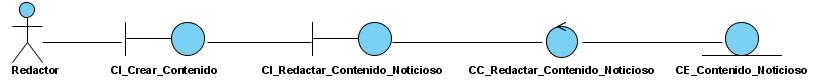
\includegraphics[width=16.5cm,height=1.8cm]{img/DCA_1}}\\
\hline
[Ver diagrama de colaboración asociado \ref{dia: dcarcn}]\\
\hline
\end{tabular}
\caption{Diagrama de clases del análisis - CU Redactar Contenido Noticioso }
\end{figure}



%TABLA VIEW_VIEW
\begin{center}
\begin{longtable}{|p{5.1cm}|p{3cm}|p{8.3cm}|}
%%para pnerle en el pie de la tabla que continua en la otra página
\multicolumn{3}{|r|}{{Continúa en la próxima página}} \\ \hline
\endfoot
% \hline
\endlastfoot

\hline

 \multicolumn{3}{|>{\columncolor[gray]{.9}}l|}{{\bf Nombre:} view\_view } \\ \hline

 \multicolumn{3}{|l|}{ {\bf Descripción:} Información básica de una vista.} \\ \hline

 nodes\_per\_block &  smallint &  Se indica el número de nodos que aparecen en cada bloque. \\ \hline

 menu\_tab\_weight &  smallint &  Se puede indicar el peso de las pestañas para ordenarlas. \\ \hline

 menu\_tab &  smallint &  Se muestra un menú de pestañas. \\ \hline

 menu &  smallint &  Se configuran las opciones para que la vista aparezca en el menú. \\ \hline

 nodes\_per\_page  &  smallint &  Cantidad de nodos por páginas. \\ \hline

 changed &  int &  Fecha en que es modificada la vista. \\ \hline

 vid &  int &  Identificador de la tabla vista. \\ \hline

 block\_footer &  long varchar &  Se indica el pie de página que tendrá la vista. \\ \hline

 block\_header &  long varchar &  Se indica el encabezado que tendrá la vista. \\ \hline

 page\_footer  &  long varchar &  Se indica el pie de página que tendrá la página de la vista en caso de que se muestre en una página. \\ \hline

  page\_empty  &  long varchar &  Indica el texto que se muestra cuando no se
encuentra ningún resultado. \\ \hline

 page\_header &  long varchar &  Se indica el encabezado que tendrá la página de la vista en caso de que se muestre en una página.\\ \hline

 block\_title & varchar &  Se cambia el título de los bloques.\\ \hline

 menu\_title & varchar &  Se indica el nombre título para el menú.\\ \hline

 url &  varchar &  En esta opción tenemos que indicar la url se quiere que tenga la vista.\\ \hline

 access &  varchar & Se indican que roles pueden consultar la vista.\\ \hline

 description &  varchar &  Se describe la vista brevemente.\\ \hline

 name &  varchar &  Indica el nombre de la vista que se va a crear.\\ \hline
\caption{Descripción de la tabla \textbf{view\_view}}
\end{longtable}
\end{center}
